\documentclass[xcolor=x11names,compress]{beamer}

%% General document %%%%%%%%%%%%%%%%%%%%%%%%%%%%%%%%%%
\usepackage{graphicx}
\usepackage{tikz}
\usetikzlibrary{decorations.fractals}
\usepackage{booktabs}
\usepackage{subfigure}
\usepackage{epstopdf}
%%%%%%%%%%%%%%%%%%%%%%%%%%%%%%%%%%%%%%%%%%%%%%%%%%%%%%


%% Beamer Layout %%%%%%%%%%%%%%%%%%%%%%%%%%%%%%%%%%
\useoutertheme[subsection=false,shadow]{miniframes}
\useinnertheme{default}
\usefonttheme{serif}
\usepackage{palatino}

\setbeamerfont{title like}{shape=\scshape}
\setbeamerfont{frametitle}{shape=\scshape}

\setbeamercolor*{lower separation line head}{bg=DeepSkyBlue4} 
\setbeamercolor*{normal text}{fg=black,bg=white} 
\setbeamercolor*{alerted text}{fg=red} 
\setbeamercolor*{example text}{fg=black} 
\setbeamercolor*{structure}{fg=black} 
 
\setbeamercolor*{palette tertiary}{fg=black,bg=black!10} 
\setbeamercolor*{palette quaternary}{fg=black,bg=black!10} 

\renewcommand{\(}{\begin{columns}}
\renewcommand{\)}{\end{columns}}
\newcommand{\<}[1]{\begin{column}{#1}}
\renewcommand{\>}{\end{column}}
%%%%%%%%%%%%%%%%%%%%%%%%%%%%%%%%%%%%%%%%%%%%%%%%%%


\graphicspath{{../optimize/figs/}{../writeup/figs/}}

\begin{document}


%%%%%%%%%%%%%%%%%%%%%%%%%%%%%%%%%%%%%%%%%%%%%%%%%%%%%%
%%%%%%%%%%%%%%%%%%%%%%%%%%%%%%%%%%%%%%%%%%%%%%%%%%%%%%

\begin{frame}
\title{Optimization Case Study}
\subtitle{CVEN5833, Optimization Techniques in Civil and Environmental Engineering}
\author{Cameron Bracken}
\date{
	\begin{tikzpicture}[decoration=Koch curve type 2] 
		\draw[DeepSkyBlue4] decorate{ decorate{ decorate{ (0,0) -- (3,0) }}}; 
	\end{tikzpicture}  
	\\
	\vspace{1cm}
	Fall, 2009.
}
\titlepage
\end{frame}

%%%%%%%%%%%%%%%%%%%%%%%%%%%%%%%%%%%%%%%%%%%%%%%%%%%%%%
%%%%%%%%%%%%%%%%%%%%%%%%%%%%%%%%%%%%%%%%%%%%%%%%%%%%%%
\section{\scshape Background}
\subsection{Motivation}
\begin{frame}{Motivation}
The town of Thirstyville is considering the use of groundwater from a local aquifur to augment their water supply.

\centering
\includegraphics[width=.6\textwidth]{site.pdf} 

\end{frame}

%%%%%%%%%%%%%%%%%%%%%%%%%%%%%%%%%%%%%%%%%%%%%%%%%%%%%%
%%%%%%%%%%%%%%%%%%%%%%%%%%%%%%%%%%%%%%%%%%%%%%%%%%%%%%
\subsection{Considerations}
\begin{frame}{Motivation}
\begin{columns}
\begin{column}{.5\textwidth}
\begin{itemize}
\item City wants optimal placement of pumps to meet demand and environmental regulations 
\item How much water can be supplied regardless of demand
\end{itemize} 
\end{column}
\begin{column}{.5\textwidth}
\includegraphics[width=\textwidth]{site.pdf} 
\end{column}
\end{columns}

\end{frame}

%%%%%%%%%%%%%%%%%%%%%%%%%%%%%%%%%%%%%%%%%%%%%%%%%%%%%%
%%%%%%%%%%%%%%%%%%%%%%%%%%%%%%%%%%%%%%%%%%%%%%%%%%%%%%
\subsection{Site Prescriptions}
\begin{frame}{Site Prescriptions}
\begin{columns}
\begin{column}{.7\textwidth}
\begin{itemize}
\item Each row (array) of pumping locations is independent
\pause
\item Pumping only at the specified locations
\pause
\item All pumps must have same capacity
\pause
\item Demand does not change frequently
\pause
\item Steady state achieved quickly relative the time scale of the water usage 
\pause
\item Drawdown affect on river level negligable
\pause
\item River level does not vary significantly
\pause
\item Minimum head
\end{itemize} 
\end{column}
\begin{column}{.3\textwidth}
\onslide\includegraphics[width=\textwidth]{site.pdf}
\end{column}
\end{columns}

\end{frame}


%%%%%%%%%%%%%%%%%%%%%%%%%%%%%%%%%%%%%%%%%%%%%%%%%%%%%%
%%%%%%%%%%%%%%%%%%%%%%%%%%%%%%%%%%%%%%%%%%%%%%%%%%%%%%
\section{Simulation Model}
\subsection{Model overview}
\begin{frame}{Model overview}

\begin{itemize}
\item Each array is modeled with a separate 1D groundwater model
\item The groundwater models are steady state  
\item East and West boundary conditions are constant (dirchlet)
\item North and South boundaries have no impact
\item Water demand is constant
\end{itemize}

\end{frame}


%%%%%%%%%%%%%%%%%%%%%%%%%%%%%%%%%%%%%%%%%%%%%%%%%%%%%%
%%%%%%%%%%%%%%%%%%%%%%%%%%%%%%%%%%%%%%%%%%%%%%%%%%%%%%
\subsection{Simulation Model Formualtion}
\begin{frame}{Simulation Model Formualtion}
The steady state simulation model for each row has the form 
$$
T\frac{\partial^2h}{\partial x^2}+\sum_iQ_i\delta(x-x_i)=0
$$
$$0\leq x\leq L$$
$$h(0)=l_j,\,\,\,\,\,h(L)=r_j$$
\end{frame}

%%%%%%%%%%%%%%%%%%%%%%%%%%%%%%%%%%%%%%%%%%%%%%%%%%%%%%
%%%%%%%%%%%%%%%%%%%%%%%%%%%%%%%%%%%%%%%%%%%%%%%%%%%%%%
\subsection{Simulation Model Solution}
\begin{frame}{Simulation Model Solution}
Using a central difference approximation
$$
A\mathbf{h}+\mathbf{f}=0
$$
A is a tridiagonal matrix.  The solution is
\pause
$$
\mathbf{h}=-A^{\mbox{-}1}\mathbf{f}.
$$
\end{frame}

%%%%%%%%%%%%%%%%%%%%%%%%%%%%%%%%%%%%%%%%%%%%%%%%%%%%%%
%%%%%%%%%%%%%%%%%%%%%%%%%%%%%%%%%%%%%%%%%%%%%%%%%%%%%%
\section{Optimization Model}
\subsection{Optimization Model Formulation}
\begin{frame}{Optimization Model Formulation}
$$\mbox{max}\,\,z=\sum_{i=1}^nh_i$$

subject to: 
\pause
$$\sum_iQ_i\geq D $$
\pause
$$h_i \geq h^* \,\,\,\forall i $$
\pause
$$0 \leq Q_i\leq Q^* \,\,\, \forall i.$$
\end{frame}

%%%%%%%%%%%%%%%%%%%%%%%%%%%%%%%%%%%%%%%%%%%%%%%%%%%%%%
%%%%%%%%%%%%%%%%%%%%%%%%%%%%%%%%%%%%%%%%%%%%%%%%%%%%%%
\section{Implementation}
\subsection{Parameters}
\begin{frame}{Parameters}
\begin{center}
\begin{tabular}{ccl}
\toprule
Parameter & Value & Dimensons\\
\midrule
T & 1 & Length$^2$/Time\\
L & 1 & Length\\
$h^*$ & .7 & Length\\
$Q^*$ & 2.5 & Volume/Time\\
$n$ & 10 & none\\
$D$ & ? & Volume/Time\\
\bottomrule
\end{tabular}
\end{center}
\end{frame}

%%%%%%%%%%%%%%%%%%%%%%%%%%%%%%%%%%%%%%%%%%%%%%%%%%%%%%
%%%%%%%%%%%%%%%%%%%%%%%%%%%%%%%%%%%%%%%%%%%%%%%%%%%%%%
\subsection{Matlab}
\begin{frame}[fragile]{Matlab}

\begin{itemize}
\item Coded in Matlab 
\begin{itemize}
	\item \texttt{fmincon}
	\item Active Set Algorithm (constrained nonlinear minimization)
	\item Needs functions to evaluate the constraints and the objective function
\end{itemize} 
\end{itemize}
\begin{verbatim}
[q,fval,exitflag,output] = fmincon(@objfun,x0,...
    ,[],[],[],[],[],@constraints,options);
\end{verbatim}

\end{frame}

%%%%%%%%%%%%%%%%%%%%%%%%%%%%%%%%%%%%%%%%%%%%%%%%%%%%%%
%%%%%%%%%%%%%%%%%%%%%%%%%%%%%%%%%%%%%%%%%%%%%%%%%%%%%%
\subsection{Linked Simulation Optimization}
\begin{frame}{Linked Simulation Optimization (LSO)}

   \centering
   \includegraphics[width=4in]{flow.pdf} 

\end{frame}

%%%%%%%%%%%%%%%%%%%%%%%%%%%%%%%%%%%%%%%%%%%%%%%%%%%%%%
%%%%%%%%%%%%%%%%%%%%%%%%%%%%%%%%%%%%%%%%%%%%%%%%%%%%%%
\subsection{Boundary Conditions}
\begin{frame}{Boundary Conditions}

\begin{columns}
\begin{column}{.4\textwidth}
3 cases and 2 sub-cases
\begin{enumerate}
\item Constant on each side 
\item Linearly decreasing downstream
\item Linear decrease, log increase
\end{enumerate} 
For each case, pumping limited() and not pumping limited. 
\end{column}
\begin{column}{.6\textwidth}
\includegraphics[width=\textwidth]{site.pdf} 
\end{column}
\end{columns}
\end{frame}


%%%%%%%%%%%%%%%%%%%%%%%%%%%%%%%%%%%%%%%%%%%%%%%%%%%%%%
%%%%%%%%%%%%%%%%%%%%%%%%%%%%%%%%%%%%%%%%%%%%%%%%%%%%%%
\subsection{Maximum Satisfiable Demand}
\begin{frame}{Maximum Satisfiable Demand (MSD)}
This is the greatest demand, $D^*$,that can be satisfied while still meeting the constraints.

$$D^*= f(h^*,Q^*)$$

For a given $h^*$ and $Q^*$, there is a unique $D^*$.

\pause The MSD is given by the unconstrained optimization problem

$$\mbox{max}\,\,D=\sum_{i=1}^nQ_i(z(D))$$

Solving for $D^*$ is an iterative process requiring multiple runs of the original optimization model.
\end{frame}

%%%%%%%%%%%%%%%%%%%%%%%%%%%%%%%%%%%%%%%%%%%%%%%%%%%%%%
%%%%%%%%%%%%%%%%%%%%%%%%%%%%%%%%%%%%%%%%%%%%%%%%%%%%%%
\section{Results}
\subsection{Case 1(a)}
\begin{frame}{Case 1(a)}

\begin{figure}[!ht]
\centering
\subfigure[Head ]{%
	\includegraphics[width=.45\textwidth]{head-constant-bounds.eps}}
\subfigure[Pumping Rates]{%
	\includegraphics[width=.45\textwidth]{pumping-constant-bounds.eps}}
\end{figure}

\end{frame}

%%%%%%%%%%%%%%%%%%%%%%%%%%%%%%%%%%%%%%%%%%%%%%%%%%%%%%
%%%%%%%%%%%%%%%%%%%%%%%%%%%%%%%%%%%%%%%%%%%%%%%%%%%%%%
\subsection{Case 1(b)}
\begin{frame}{Case 1(b)}

\begin{figure}[!ht]
\centering
\subfigure[Head ]{%
	\includegraphics[width=.45\textwidth]{head-constant-bounds-minq.eps}}
\subfigure[Pumping Rates]{%
	\includegraphics[width=.45\textwidth]{pumping-constant-bounds-minq.eps}}
\end{figure}

\end{frame}

%%%%%%%%%%%%%%%%%%%%%%%%%%%%%%%%%%%%%%%%%%%%%%%%%%%%%%
%%%%%%%%%%%%%%%%%%%%%%%%%%%%%%%%%%%%%%%%%%%%%%%%%%%%%%
\subsection{Case 2(a)}
\begin{frame}{Case 2(a)}

\begin{figure}[!ht]
\centering
\subfigure[Head]{%
	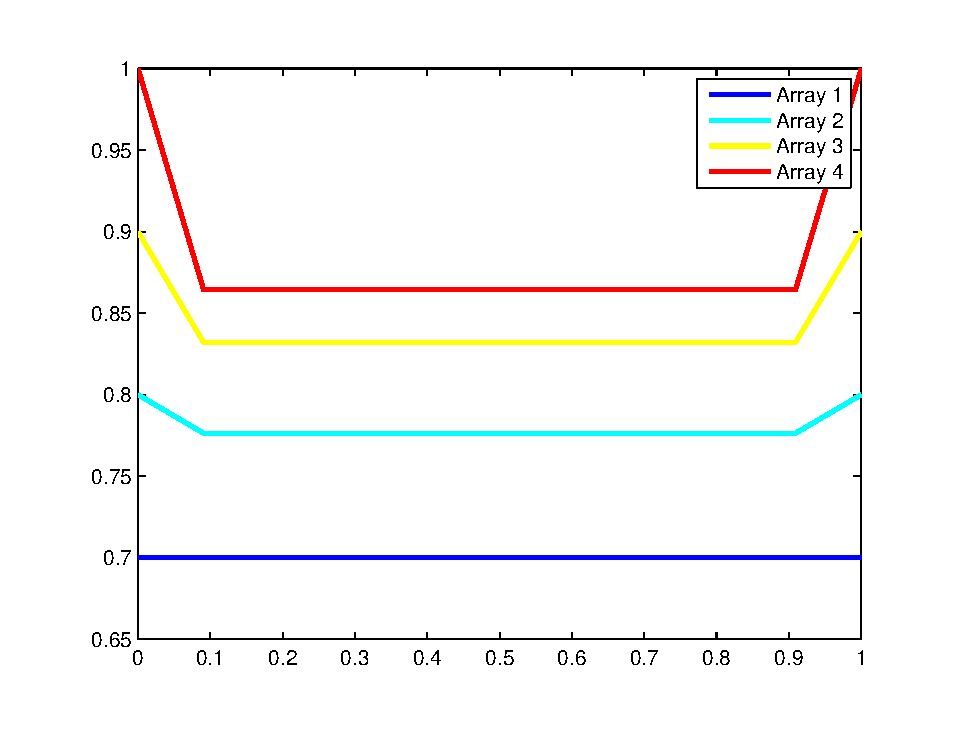
\includegraphics[width=.45\textwidth]{head-linear-bounds.eps}}
\subfigure[Pumping Rates]{%
	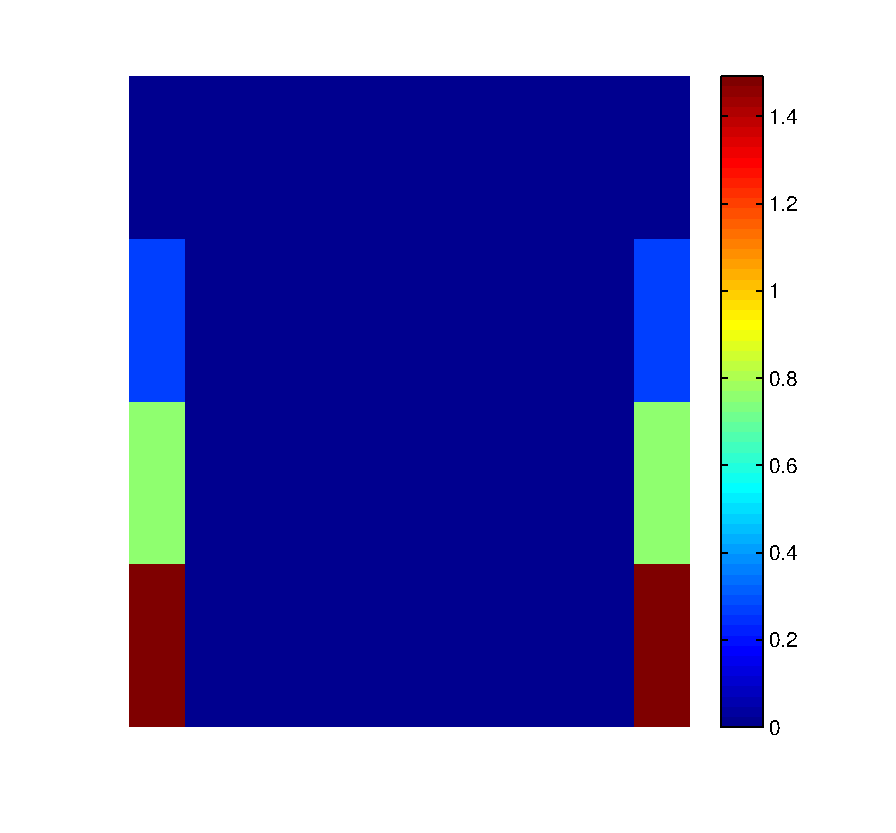
\includegraphics[width=.45\textwidth]{pumping-linear-bounds.eps}}
\end{figure}

\end{frame}


%%%%%%%%%%%%%%%%%%%%%%%%%%%%%%%%%%%%%%%%%%%%%%%%%%%%%%
%%%%%%%%%%%%%%%%%%%%%%%%%%%%%%%%%%%%%%%%%%%%%%%%%%%%%%
\subsection{Case 2(b)}
\begin{frame}{Case 2(b)}

\begin{figure}[!ht]
\centering
\subfigure[Head]{%
	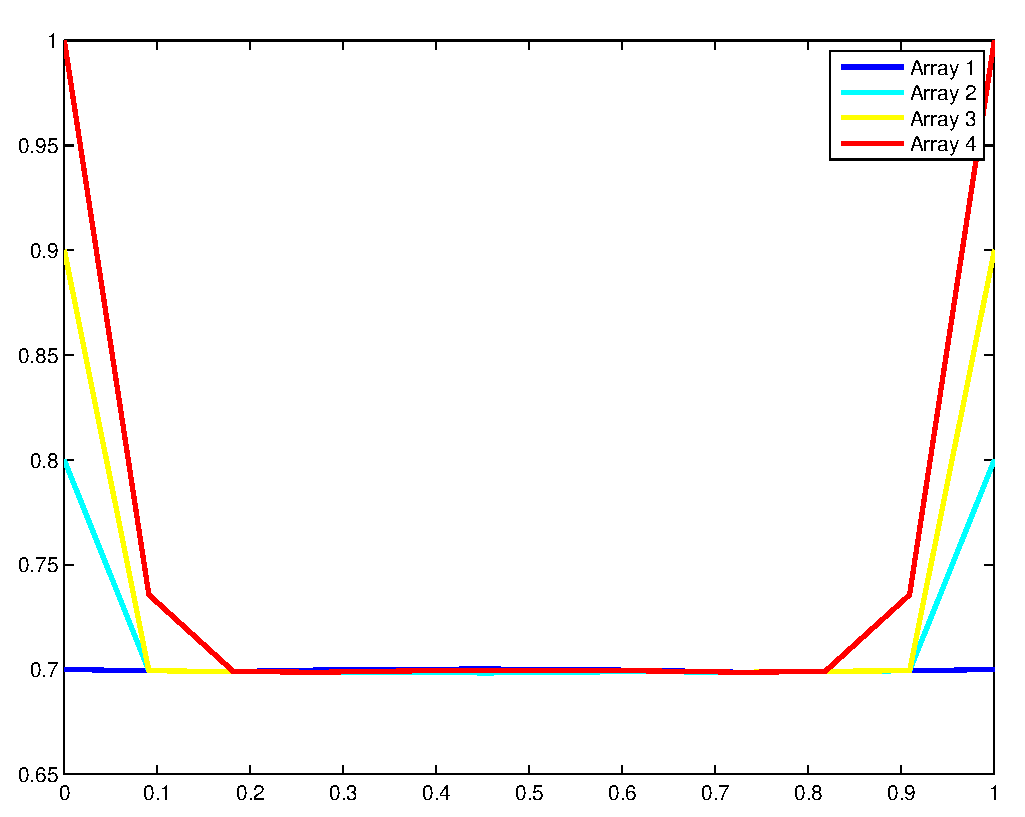
\includegraphics[width=.45\textwidth]{head-linear-bounds-minq.eps}}
\subfigure[Pumping Rates]{%
	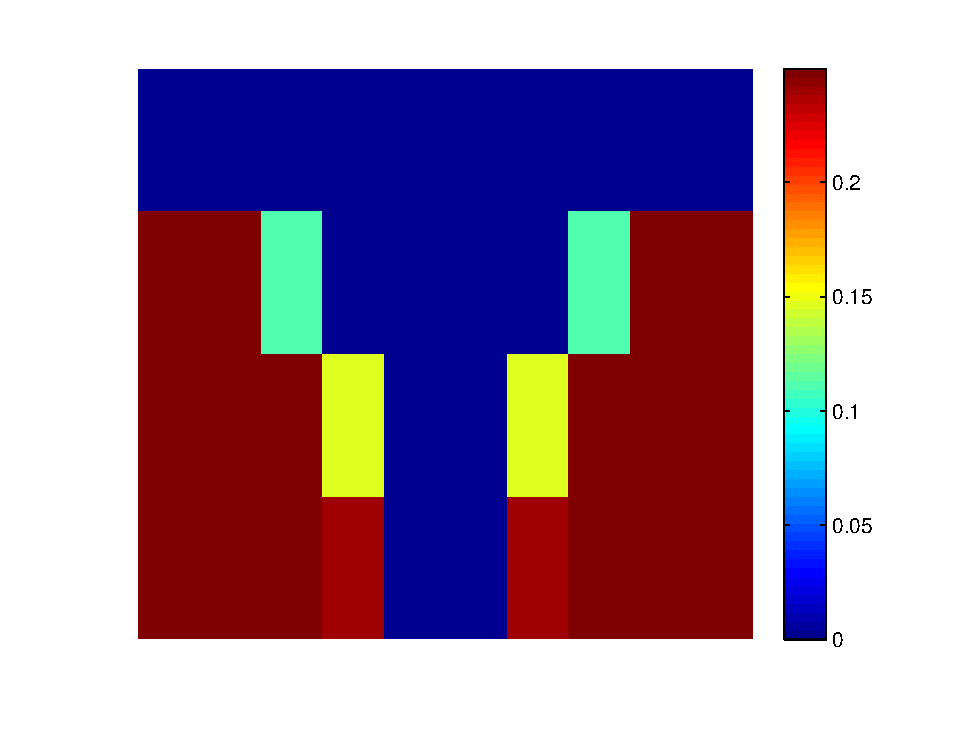
\includegraphics[width=.45\textwidth]{pumping-linear-bounds-minq.eps}}
\end{figure}

\end{frame}

%%%%%%%%%%%%%%%%%%%%%%%%%%%%%%%%%%%%%%%%%%%%%%%%%%%%%%
%%%%%%%%%%%%%%%%%%%%%%%%%%%%%%%%%%%%%%%%%%%%%%%%%%%%%%
\subsection{Case 3(a)}
\begin{frame}{Case 3(a)}

\begin{figure}[!ht]
\centering
\subfigure[Head]{%
	\includegraphics[width=.45\textwidth]{head-log-bounds.eps}}
\subfigure[Pumping Rates]{%
	\includegraphics[width=.45\textwidth]{pumping-log-bounds.eps}}
\end{figure}

\end{frame}


%%%%%%%%%%%%%%%%%%%%%%%%%%%%%%%%%%%%%%%%%%%%%%%%%%%%%%
%%%%%%%%%%%%%%%%%%%%%%%%%%%%%%%%%%%%%%%%%%%%%%%%%%%%%%
\subsection{Case 3(b)}
\begin{frame}{Case 3(b)}

\begin{figure}[!ht]
\centering
\subfigure[Head]{%
	\includegraphics[width=.45\textwidth]{head-log-bounds-minq.eps}}
\subfigure[Pumping Rates]{%
	\includegraphics[width=.45\textwidth]{pumping-log-bounds-minq.eps}}
\end{figure}

\end{frame}

%%%%%%%%%%%%%%%%%%%%%%%%%%%%%%%%%%%%%%%%%%%%%%%%%%%%%%
%%%%%%%%%%%%%%%%%%%%%%%%%%%%%%%%%%%%%%%%%%%%%%%%%%%%%%
\subsection{MSD Results}
\begin{frame}{MSD Results}
Optimal solution as a function of demand.
\begin{center}
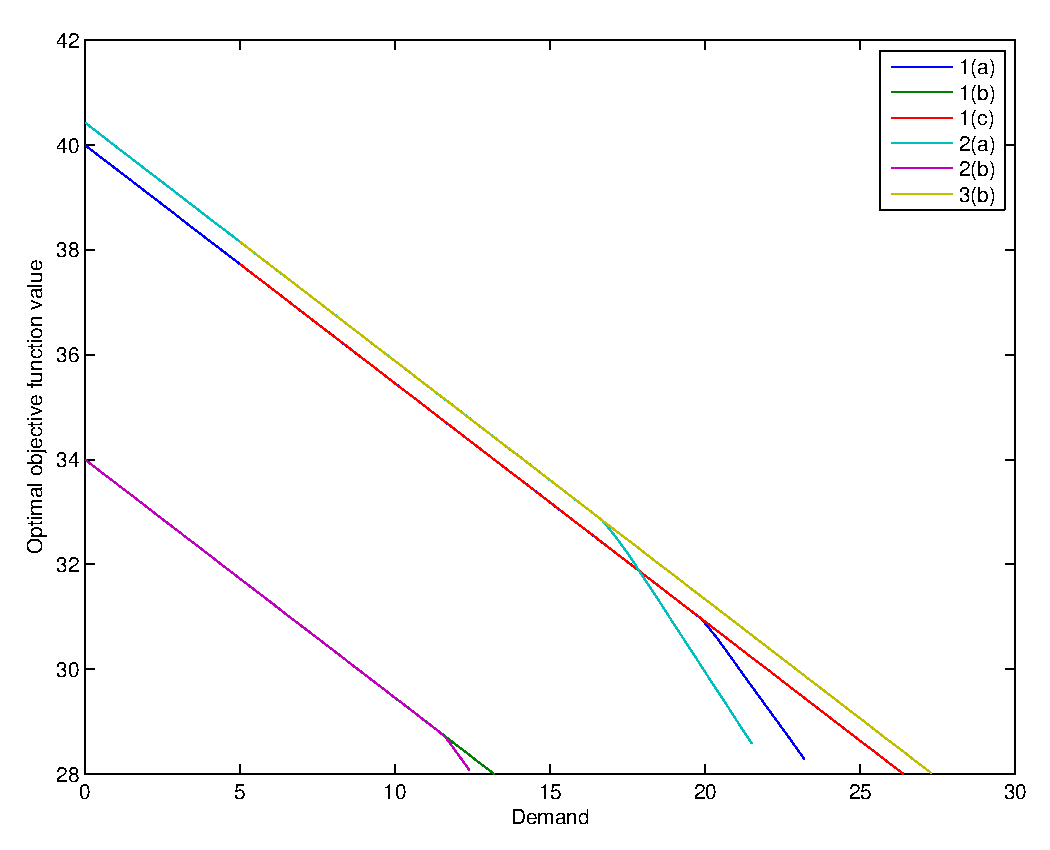
\includegraphics[width=.7\textwidth]{../optimize/figs/allzvd.eps}
\end{center}
\end{frame}

%%%%%%%%%%%%%%%%%%%%%%%%%%%%%%%%%%%%%%%%%%%%%%%%%%%%%%
%%%%%%%%%%%%%%%%%%%%%%%%%%%%%%%%%%%%%%%%%%%%%%%%%%%%%%
\section{Conclusion}
\subsection{Conclusions}
\begin{frame}{Conclusions}

\begin{itemize}
	\item Hypothetical aquifer
	\pause
	\item Linked Simulation Optimization methodology
	\pause
	\item Useful to think in terms of Maximum Satisfiable Demand
	\pause
	\item Results are intuitive, should do a full sensitivity analysis
\end{itemize} 

\end{frame}

\end{document}


